% Single-qubit data re-uploading classifier (Perez-Salinas et al., Quantum 4, 226 (2020), Fig. 2 and Eq. (5)).
% Top: data upload U(x) followed by a trainable rotation U(phi_i), repeated L times.
% Bottom: compressed layer U(theta_i + w_i o x), a ZYZ rotation with angles linear in the data.
% Readout: fidelities F_c = |<psi_c|psi(x)>|^2 with the label states.
\documentclass[tikz,border=4pt]{standalone}
\usepackage{amsmath,amssymb}
\usetikzlibrary{quantikz}
\begin{document}
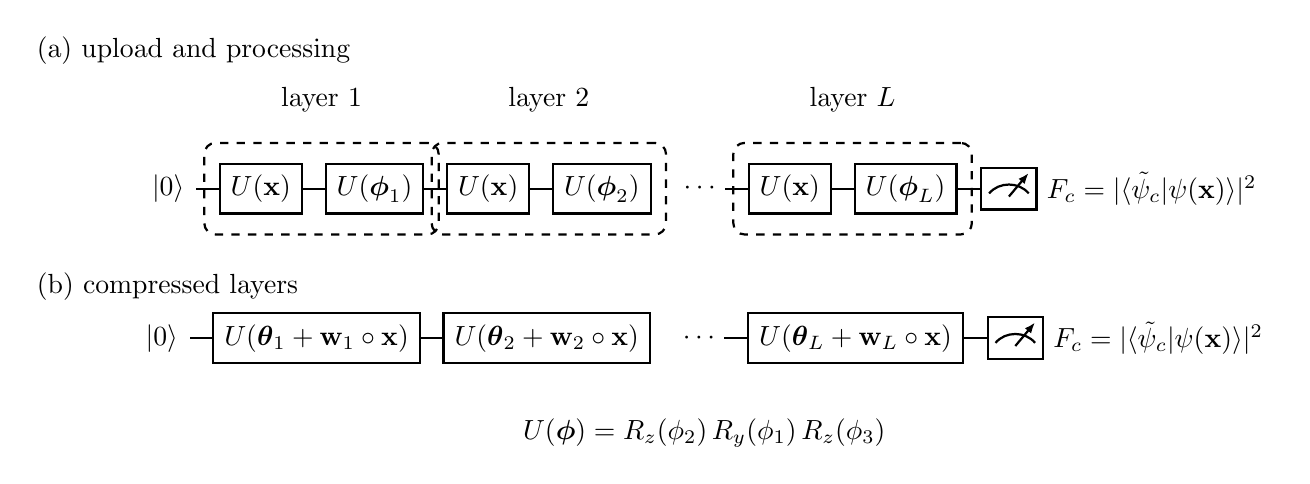
\begin{tikzpicture}
\node at (0,0) {\begin{quantikz}[row sep=0.3cm, column sep=0.3cm]
\lstick{$\ket{0}$} & \gate{U(\mathbf x)}\gategroup[1,steps=2,style={dashed,rounded corners,inner xsep=2pt},background,label style={label position=above,anchor=south,yshift=0.05cm}]{layer $1$} & \gate{U(\boldsymbol\phi_1)} & \gate{U(\mathbf x)}\gategroup[1,steps=2,style={dashed,rounded corners,inner xsep=2pt},background,label style={label position=above,anchor=south,yshift=0.05cm}]{layer $2$} & \gate{U(\boldsymbol\phi_2)} & \ \cdots\ & \gate{U(\mathbf x)}\gategroup[1,steps=2,style={dashed,rounded corners,inner xsep=2pt},background,label style={label position=above,anchor=south,yshift=0.05cm}]{layer $L$} & \gate{U(\boldsymbol\phi_L)} & \meter{} \rstick{$F_c=|\langle\tilde\psi_c|\psi(\mathbf x)\rangle|^2$}
\end{quantikz}};
\node at (0,-2.3) {\begin{quantikz}[row sep=0.3cm, column sep=0.3cm]
\lstick{$\ket{0}$} & \gate{U(\boldsymbol\theta_1+\mathbf w_1\circ\mathbf x)} & \gate{U(\boldsymbol\theta_2+\mathbf w_2\circ\mathbf x)} & \ \cdots\ & \gate{U(\boldsymbol\theta_L+\mathbf w_L\circ\mathbf x)} & \meter{} \rstick{$F_c=|\langle\tilde\psi_c|\psi(\mathbf x)\rangle|^2$}
\end{quantikz}};
\node[anchor=west] at (-8.6,1.35) {(a) upload and processing};
\node[anchor=west] at (-8.6,-1.65) {(b) compressed layers};
\node at (0,-3.5) {$U(\boldsymbol\phi)=R_z(\phi_2)\,R_y(\phi_1)\,R_z(\phi_3)$};
\end{tikzpicture}
\end{document}
